\begin{frame}{Simplex space}
\only<1>{
\note{
In this presentation, I will frequently refer to simplex space. 
A simplex space is collection of vectors with non-negative values that always sum to a constant.
This space is known as the \emph{simplex} and it is common to set \( k = 1 \).
We refer to data from this space as \emph{compositional data}.
}

\vspace{1em}

A simplex is a convex space of all vectors with non-negative components that sum to a constant. 

\begin{center}
\colorbox{blue!10}{\parbox{0.8\textwidth}{
\begin{center}
\[
S^c_k = \left\{ (y_1, \dots, y_k)^\top \in \mathbb{R}^k \,\middle|\, y_i \geq 0, \ \sum_{i=1}^k y_i = \textcolor{blue}{c} \right\}
\]
\end{center}
}}
\end{center}

It is common to set \(  \textcolor{blue}{c = 1} \). We refer to data from this space as \emph{compositional data}.
}

\only<2>{
\note{Another important space in the context of compositional data is the Aitchison space. This space is a log-transformed version of the simplex. Another important log-ratio transformation is the isometric log-ratio (ILR) transformation.
In reality, there is a wide variety of log-ratio transformations of the simplex space. }
Aitchison space:
\begin{center}
\colorbox{blue!10}{\parbox{1\textwidth}{
\begin{center}
\[
A_k = \left\{\left(\ln\!\left(\frac{Y_1}{g(\mathbf{Y})}\right), \ldots, \ln\!\left(\frac{Y_{k}}{g(\mathbf{Y})}\right)\right); g(\mathbf{Y}) = \left(\prod_{i=1}^{k} Y_i\right)^{1/{k}}\right\}
\]
\end{center}
}}
\end{center}
}
\end{frame}


\begin{frame}{Compositional data}
\only<1>{
\note{
Consider a vector with \(K\) components, where the only constraint is that all components are non-negative. Two important transformations of this vector are the following vectors. 

1. transform data to simplex space

2. transform data to Aitchison space

so we have original vector, simplex vector and Aitchison vector.

In general, the original vector \(\mathbf{Y} = (Y_1, \ldots, Y_K) \in \mathbb{R}_+^K\) cannot be recovered from these transformations, because they remove information about the absolute scale of the components. However, the simplex representation and the Aitchison representation can be recovered from one another.

There are some challenges in interpreting results that are based on the Simplex or Aitchison space.
}

Consider a vector \(\mathbf{Y} = (Y_1, Y_2, \ldots, Y_k) \in \mathbb{R}_+^k\). Two commonly used transformations of \(\mathbf{Y}\) are of particular interest:  

\begin{equation*}
\mathbf{S}_{k}(\mathbf{Y}) = \left(\frac{Y_1}{\sum_{i=1}^{k} Y_i}, \ldots, \frac{Y_{k}}{\sum_{i=1}^{k} Y_i}\right),
\end{equation*}

and  

\begin{equation*}
\mathbf{A}_{k}(\mathbf{Y}) = \left(\ln\!\left(\frac{Y_1}{g(\mathbf{Y})}\right), \ldots, \ln\!\left(\frac{Y_{k}}{g(\mathbf{Y})}\right)\right),
\end{equation*}

where \(g(\mathbf{Y}) = \left(\prod_{i=1}^{k} Y_i\right)^{1/{k}}\) denotes the geometric mean of \(\mathbf{Y}\). 
}

\only<2>{
\note{
it is simplest case of these two spaces.
}
Consider a vector \(\mathbf{Y} = (Y_1, Y_2) \in \mathbb{R}_+^2\). 

\begin{equation*}
\mathbf{S}(\mathbf{Y}) = \left(\frac{Y_1}{Y_1+Y_2},  \frac{Y_2}{Y_1+Y_2}\right),
\end{equation*}

and  

\begin{equation*}
\mathbf{A}(\mathbf{Y}) = \left(\frac{1}{2}\ln\!\left(\frac{Y_1}{Y_2}\right), \frac{1}{2}\ln\!\left(\frac{Y_2}{Y_1}\right)\right),
\end{equation*}

where \(g(\mathbf{Y}) = \left(\prod_{i=1}^2 Y_i\right)^{1/2}\) denotes the geometric mean of \(\mathbf{Y}\). 
}

\only<3>{
\note{
One important point is that the correlation between components 1 and 2 is \(-1\) in both the simplex and the Aitchison space, no matter what the correlation between \(Y_1\) and \(Y_2\) is.

this type correlation between components in the simplex or in the Aitchison space should \textbf{not} be interpreted as the correlation between the original components of \(\mathbf{Y}\). 

This is also true for higher dimensions. The correlations in these spaces can be far from zero, even when the true correlation between \(Y_1\) and \(Y_2\) is zero.
}

\textbf{Spurious correlations:} Based on Pearson (1897), correlations between the components of $\mathbf{S}(\mathbf{Y})$ or $\mathbf{A}(\mathbf{Y})$ should \textbf{not} be interpreted as correlations between the components of $\mathbf{Y}$.  

For example, 
\[
\boxed{
\begin{aligned}
&\text{cor}\left(\frac{Y_1}{Y_1 + Y_2}, \frac{Y_2}{Y_1 + Y_2}\right) = -1 \\[1em]
&\text{cor}\left(\frac{1}{2}\ln\left(\frac{Y_1}{Y_2}\right), \frac{1}{2}\ln\left(\frac{Y_2}{Y_1}\right)\right) = -1
\end{aligned}
}
\quad \Longrightarrow \quad \text{cor}(Y_1, Y_2) = 0
\]
}

\only<4>{
\note{
Pearson (1897) referred to this as \textit{spurious correlations}. His work marks the starting point of a long and ongoing effort to answer the following challenging question:

Which of the two transformations, simplex or Aitchison, provides the most desirable properties for statistical analysis and modeling?

After Pearson, many researchers argued that these spurious correlations happen because Euclidean metrics are not appropriate for the simplex. Surprisingly, they only refer to the simplex space, not the Aitchison space. But in both spaces the correlations are still spurious.
}

\textbf{Spurious correlations:}
\[
\boxed{
\begin{aligned}
&\text{cor}\left(\frac{Y_1}{\sum_{i=1}^{K} Y_i}, \frac{Y_2}{\sum_{i=1}^{K} Y_i}\right) \neq 0 \\[1em]
&\text{cor}\left(\frac{Y_1}{g(\mathbf{Y})}, \frac{Y_2}{g(\mathbf{Y})}\right) \neq 0
\end{aligned}
}
\quad \Longrightarrow \quad \text{cor}(Y_1, Y_2) = 0
\]

\textbf{\textcolor{blue}{Question}}: Which of the two transformations, \(\mathbf{s}(\mathbf{Y})\) or \(\mathbf{a}(\mathbf{Y})\), offers the most desirable properties for statistical analysis and modeling?
}

\only<5>{
\note{
I want to emphasize that the claim that ``Euclidean metrics are the problem'' is not correct. There is no mathematical problem that needs to be fixed. These spurious correlations are actually expected and understandable. We just need to be careful with how we interpret them.

This controversy and misunderstandings has had a negative effect on the proper development of methods for compositional data. As a result, the methodology for working directly in the simplex space has not been well explored.

However as we worked through literature we became convinced to focus on working directly in the simplex space, especially from a machine learning point of view.
}

\colorbox{green!10}{\parbox{0.95\textwidth}{
\[
\begin{aligned}
\operatorname{cor}\!\left(\frac{Y_1}{Y_1 + Y_2}, \frac{Y_2}{Y_1 + Y_2}\right)
=&
\operatorname{cor}\!\left(\frac{Y_1}{Y_1 + Y_2}, 1 - \frac{Y_1}{Y_1 + Y_2}\right)\\
= &
\operatorname{cor}\!\left(f(Y_1, Y_2),\, 1 - f(Y_1, Y_2)\right)
= -1.
\end{aligned}
\]
}}
}
\end{frame}


\begin{frame}{}
\only<1>{ 
\note{I want to quickly talk about the advantages of these two spaces.}

\textbf{\textcolor{blue}{Question}}: Which of the two transformations, \(\mathbf{s}(\mathbf{Y})\) or \(\mathbf{a}(\mathbf{Y})\), offers more desirable properties for statistical analysis and modeling.
}

\only<2>{ 
\note{One obvious advantage of the simplex space is that we can easily understand what each component represents. For example, suppose a class has 50 Mathematics, 100 Statistics, and 150 Computer Science students. In the simplex space, we can immediately say that, for instance, \(0.17\) of the students are from the Mathematics department.

In contrast, an Aitchison-transformed vector might give a value such as \(-0.6\), which has no direct, intuitive interpretation. To understand the meaning of such numbers, we must transform the vector back to the simplex space. Only then can the components be interpreted in terms of proportions or relative contributions.
}

\textbf{\textcolor{blue}{Advantage of \(\mathbf{s}(\mathbf{Y})\):}}

The advantage of $\mathbf{s}(\mathbf{Y})$ is its interpretability.

Example, consider 
\(
\mathbf{Y} = (50, 150, 100),
\)
represents the number of students in mathematics, statistics, and computer science in a class.  

Then
\begin{align*}
\mathbf{s}(\mathbf{Y}) 
&=\scalebox{1.2}{$\left(\frac{50}{50+150+100},\;\frac{150}{50+150+100},\;\frac{100}{50+150+100}\right)$} \\
&= (0.17, 0.50, 0.33), \\[6pt]
\mathbf{a}(\mathbf{Y})
&= \scalebox{1.1}{$\left(
\ln \frac{50}{(50 \times 150 \times 100)^{1/3}},\;\ 
\ln \frac{150}{(50 \times 150 \times 100)^{1/3}},\;\ 
\ln \frac{100}{(50 \times 150 \times 100)^{1/3}}
\right)$} \\
&= (-0.60, 0.50, 0.10).
\end{align*}

However, the components of $\mathbf{a}(\mathbf{Y})$ are not easy to interpret directly (e.g., $-0.60$), so we usually transform them back to the compositional scale $\mathbf{s}(\mathbf{Y})$ for intuitive understanding.
}

\only<3>{ 
\note{
The important practical advantage of Aitchison space is that it maps compositional data to the real space \(\mathbb{R}^K\), giving us more flexibility.

In fact, this is the only practical advantage of Aitchison space that I am aware of and have used it many times in my own work.
}

\textbf{\textcolor{blue}{Advantage of \(\mathbf{a}(\mathbf{Y})\):}} 

The practical and important advantage is that it maps the data to real space $\mathbb{R}$, enabling the use of standard distributions and widely available libraries. 
    
\medskip

\textbf{Principles of CoDA (\textcolor{red}{Ambiguous perspective):}}

One major development is the Principles of Compositional Data Analysis (CoDA), designed to support the use of $\mathbf{a}(\mathbf{Y})$.
}
\end{frame}




\begin{frame}{}
\only<1>{
\texttt{\textcolor{blue}{method}}: What is this parameter for?

\note{One important disadvantage of this approach is the computational cost of estimating the maximum likelihood parameters.

Because there’s no closed-form solution for the maximum likelihood estimator of the Dirichlet distribution parameters we have to solve it numerically.

For example, if we have 10 covariates and 10 candidate split points per covariate, that means we need to numerically solve the MLE problem 600 times at each node.

When computational performance is important, we can change the default estimation method from MLE to MoM.
}
\centering
\begin{tikzpicture}[
  node distance=1cm and 1.5cm,
  every node/.style={font=\small},
  data/.style={rectangle, draw, align=center, fill=blue!5, rounded corners, inner sep=5pt},
  split/.style={->, thick}
  ]
  % Parent node
  \node[data] (parent) {
    \textbf{Parent Node} \\[0.15cm]
    Data: $X^{n \times m}$, $Y^{n \times k}$
  };
  
  % Left child
  \node[data, below left=of parent] (left) {
    Data: $X^{n_1 \times m}$, $Y^{n_1 \times k}$ \\[0.15cm]
    $\mathcal{L}(Y^{n_1 \times k}, \alpha_1^L, \alpha_2^L, \alpha_3^L)$
  };
  
  % Right  
  \node[data, below right=of parent] (right) {
    Data: $X^{n_2 \times m}$, $Y^{n_2 \times k}$ \\[0.15cm]
    $\mathcal{L}(Y^{n_2 \times k}, \alpha_1^R, \alpha_2^R, \alpha_3^R)$
  };
  
  % Arrows
  \draw[split] (parent) -- node[midway, left] {$x_{ij} \leq c$} (left);
  \draw[split] (parent) -- node[midway, right] {$x_{ij} > c$} (right);
\end{tikzpicture}

\vspace{0.5cm}



\[
(i^*, c^*) = \operatorname{argmax}_{i,c} \left( \max_{\boldsymbol{\alpha}^L} \mathcal{L}(Y^{n_1 \times k}, \boldsymbol{\alpha}^L) + \max_{\boldsymbol{\alpha}^R} \mathcal{L}(Y^{n_2 \times k}, \boldsymbol{\alpha}^R) \right)
\]
\textbf{Parameter Estimation Complexity:} $6 \times m \times p$ parameters per split:
\[
\text{Total = }6 \times m \times p =  6 \times 10 \times 10 = 600 \text{ optimizations per node}
\]
}
% \only<2>{
% For trees that can potentially grow in all directions to at least 6 levels deep, we have:
% \begin{equation}
% 3 \times m \times p \times \sum_{i=1}^{6} 2^i = 3 \times m \times p \times 126 = 378 \times m \times p
% \end{equation}
% parameters that we estimate dynamically. This number can become very large---for example, when $m=10$ and $p=10$, the total number of parameters is $378 \times 10 \times 10 = 37,800$.
% }
\only<2>{
\note{If we build a tree with just three levels — meaning a tree with 8 leaves — we already need to solve the optimization problem 4,200 times.

This is a large computational cost. And remember, trees can grow much deeper depending on the dataset. As the depth increases, the number of nodes — and therefore the number of parameter estimations — grows exponentially.}

    \centering
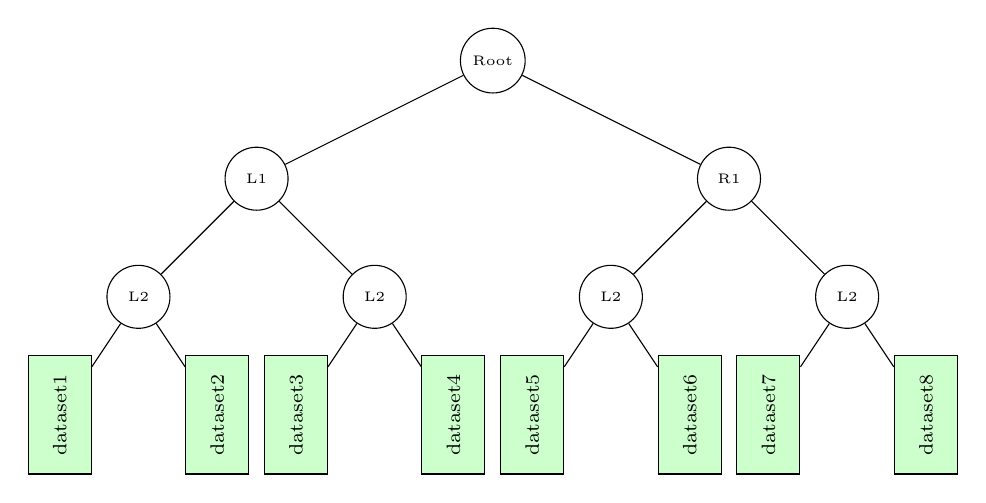
\begin{tikzpicture}[
  level/.style={sibling distance=60mm/#1},
  every node/.style={circle, draw, minimum size=8mm, font=\tiny},
  leaf/.style={rectangle, draw, fill=green!20, minimum width=15mm, minimum height=8mm, font=\scriptsize, rotate=90}
]
\node {Root}
  child {
    node {L1}
    child {
      node {L2}
      child {
        node[leaf] {dataset1}
      }
      child {
        node[leaf] {dataset2}
      }
    }
    child {
      node {L2}
      child {
        node[leaf] {dataset3}
      }
      child {
        node[leaf] {dataset4}
      }
    }
  }
  child {
    node {R1}
    child {
      node {L2}
      child {
        node[leaf] {dataset5}
      }
      child {
        node[leaf] {dataset6}
      }
    }
    child {
      node {L2}
      child {
        node[leaf] {dataset7}
      }
      child {
        node[leaf] {dataset8}
      }
    }
  };
\end{tikzpicture}

With $10$ covariates and $10$ candidates per covariate, the model requires $3 \times 10\times 10 \times (2+2^2+2^3) = 4200$ parameters, all estimated using maximum likelihood estimation. As the tree depth increases, the parameter count grows exponentially.
\note{
This tree diagram illustrates a hierarchical model designed to generate 8 subdatasets, each following a Dirichlet distribution. With 10 covariates and 10 candidates per covariate, the model requires 10×10×(2+2²+2³) = 1,400 parameters, all estimated using maximum likelihood estimation. As the tree depth increases, the parameter count grows exponentially.}
}









\only<3>{
\note{}
\boxed{
store\_samples = TRUE}
    \centering
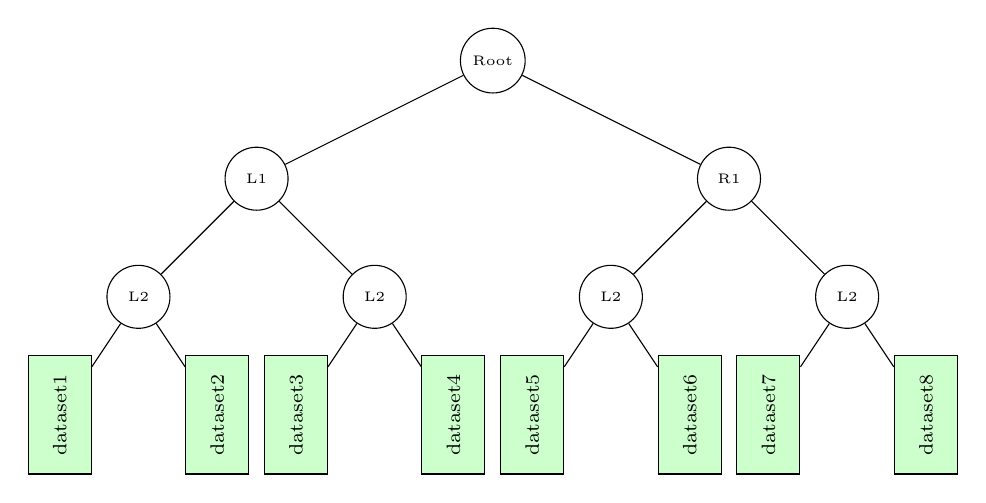
\begin{tikzpicture}[
  level/.style={sibling distance=60mm/#1},
  every node/.style={circle, draw, minimum size=8mm, font=\tiny},
  leaf/.style={rectangle, draw, fill=green!20, minimum width=15mm, minimum height=8mm, font=\scriptsize, rotate=90}
]
\node {Root}
  child {
    node {L1}
    child {
      node {L2}
      child {
        node[leaf] {dataset1}
      }
      child {
        node[leaf] {dataset2}
      }
    }
    child {
      node {L2}
      child {
        node[leaf] {dataset3}
      }
      child {
        node[leaf] {dataset4}
      }
    }
  }
  child {
    node {R1}
    child {
      node {L2}
      child {
        node[leaf] {dataset5}
      }
      child {
        node[leaf] {dataset6}
      }
    }
    child {
      node {L2}
      child {
        node[leaf] {dataset7}
      }
      child {
        node[leaf] {dataset8}
      }
    }
  };
\end{tikzpicture}


\note{
}
}

\only<4>{
\note{}
\boxed{
store\_samples = FALSE}
    \centering
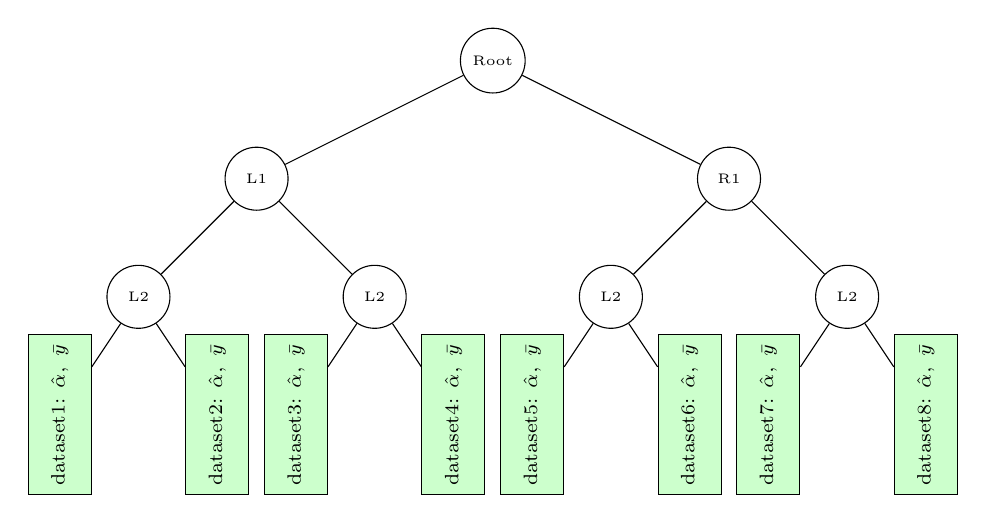
\begin{tikzpicture}[
  level/.style={sibling distance=60mm/#1},
  every node/.style={circle, draw, minimum size=8mm, font=\tiny},
  leaf/.style={rectangle, draw, fill=green!20, minimum width=15mm, minimum height=8mm, font=\scriptsize, rotate=90}
]
\node {Root}
  child {
    node {L1}
    child {
      node {L2}
      child {
        node[leaf] {dataset1: $\hat{\alpha},\,\, \bar{y}$}
      }
      child {
        node[leaf] {dataset2: $\hat{\alpha},\,\, \bar{y}$}
      }
    }
    child {
      node {L2}
      child {
        node[leaf] {dataset3: $\hat{\alpha},\,\, \bar{y}$}
      }
      child {
        node[leaf] {dataset4: $\hat{\alpha},\,\, \bar{y}$}
      }
    }
  }
  child {
    node {R1}
    child {
      node {L2}
      child {
        node[leaf] {dataset5: $\hat{\alpha},\,\, \bar{y}$}
      }
      child {
        node[leaf] {dataset6: $\hat{\alpha},\,\, \bar{y}$}
      }
    }
    child {
      node {L2}
      child {
        node[leaf] {dataset7: $\hat{\alpha},\,\, \bar{y}$}
      }
      child {
        node[leaf] {dataset8: $\hat{\alpha},\,\, \bar{y}$}
      }
    }
  };
\end{tikzpicture}

}
\end{frame}


% \only<4>{

%  This large parameter space provides the model with sufficient flexibility to accommodate diverse datasets, addressing a key limitation of traditional methods related to the Dirichlet distribution, like Dirichlet regression methods for compositional data analysis. However, this flexibility comes at a significant computational cost, rendering the approach impractical for large-scale datasets. 
% }
% \only<3>{
% The discussion of computational performance remains a significant issue for big datasets in our methodology. We have identified several promising directions for future research and performance improvements. As we discussed, MoM works well as an alternative to MLE, providing good approximations with higher computational speed. We can combine these estimation methods by selectively replacing MLE with MoM in specific nodes where we can predict the results of both methods would be similar, rather than applying MoM to all nodes.
% }



\begin{frame}
\frametitle{Distributional Dirichlet Random Forests (DRF)}
\note{
Another idea that I really like is to fit an empirical probability function.

Actually, we can fit a probability function on the training dataset. Then, for a new observation, we can evaluate this probability function to obtain its predicted distribution.

Actually, we can fit a probability function on the training dataset. This method was introduced in 2022. I will not go into the details of how it works. I have a simple example to explain it, but I will skip it to save time.
}

\begin{equation*}
P(Y = y_i \mid X = \mathbf{x}_{\text{new}}) = w_i(\mathbf{x}_{\text{new}}), \quad i = 1, \dots, n, \quad \sum_{i=1}^{n} w_i(\mathbf{x}_{\text{new}}) = 1.
\end{equation*}

\vspace{0.5em}
\begin{block}{}
The formula for the normalized weight $w_i$ is:
\[
w_i(\mathbf{x}_{\text{new}})
= \frac{1}{B} \sum_{k=1}^B 
\frac{\mathbf{1}\!\left(\mathbf{x}_{\text{new}} \in L_k(i)\right)}{|L_k(i)|}.
\]
where $|L_k(i)|$ is the size of the terminal node in tree $k$ where $\mathbf{x}_{\text{new}}$ falls.
\end{block}
\end{frame}


\begin{frame}
\frametitle{Example: Distributional Weight Calculation}
\only<1>{
\note{
Instead of explaining the full formula, let's consider a simple example. Suppose in the random forest we have only two trees, and a new observation falls into a specific leaf in each tree.  

For the first tree, the conditional probability is \(1/3\) for observations in that leaf and zero for observations not in the leaf.  
For the second tree, the conditional probability is \(1/2\).  

The final probability for the new observation is obtained by averaging over the trees.
}

\framesubtitle{Calculating weights $w_i$ for a new observation $\mathbf{x}_{\text{new}}$}

Assume $\mathbf{x}_{\text{new}}$ falls into the specified terminal nodes in $B=2$ trees.

\vspace{0.2cm}
\begin{columns}
\column{0.45\textwidth}
\centering
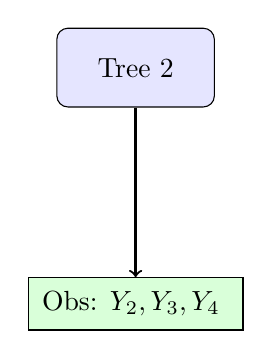
\begin{tikzpicture}[
  node distance=0.15cm,
  data/.style={rectangle, draw, align=center, fill=blue!10, minimum width=2cm, minimum height=1cm, rounded corners},
  leaf/.style={rectangle, draw, align=center, fill=green!15, minimum width=2.5cm, inner sep=5pt}
  ]
  
  \node[data] (root2) at (4, 3) {Tree 2};
  \node[leaf] (leaf2) at (4, 0) {
    Obs: $Y_2, Y_3,Y_4$
  };
  \draw[->, thick] (root2) -- (leaf2);
\end{tikzpicture}

\[
P(Y = y_i \mid \mathbf{x}_{\text{new}}) = \frac{1}{3} \, \mathbf{1}_{i \in \{2,3,4\}}
\]

\column{0.55\textwidth}
\centering
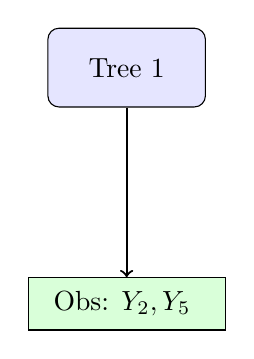
\begin{tikzpicture}[
  node distance=0.15cm,
  data/.style={rectangle, draw, align=center, fill=blue!10, minimum width=2cm, minimum height=1cm, rounded corners},
  leaf/.style={rectangle, draw, align=center, fill=green!15, minimum width=2.5cm, inner sep=5pt}
  ]
  
  \node[data] (root1) at (0, 3) {Tree 1};
  \node[leaf] (leaf1) at (0, 0) {
    Obs: $Y_2, Y_5$
  };
  \draw[->, thick] (root1) -- (leaf1);
\end{tikzpicture}

\[
P(Y = y_i \mid \mathbf{x}_{\text{new}}) = \frac{1}{2} \, \mathbf{1}_{i \in \{2,5\}}
\]
\end{columns}
}

\only<2>{
\note{
Instead of explaining the full formula, let's consider a simple example. Suppose in the random forest we have only two trees, and a new covariate falls into a specific leaf in each tree.  

For the first tree, the conditional probability is \(1/3\) for observations in that leaf and zero for observations not in the leaf.  
For the second tree, the conditional probability is \(1/2\).  

The final probability for the new observation is obtained by averaging over the trees.
}

\framesubtitle{Calculating weights $w_i$ for a new observation $\mathbf{x}_{\text{new}}$}

Assume $\mathbf{x}_{\text{new}}$ falls into the specified terminal nodes in $B=2$ trees.

\vspace{0.2cm}
\begin{columns}
\column{0.45\textwidth}
\centering
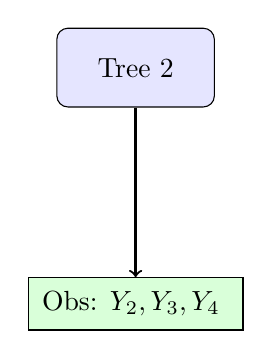
\begin{tikzpicture}[
  node distance=0.15cm,
  data/.style={rectangle, draw, align=center, fill=blue!10, minimum width=2cm, minimum height=1cm, rounded corners},
  leaf/.style={rectangle, draw, align=center, fill=green!15, minimum width=2.5cm, inner sep=5pt}
  ]
  
  \node[data] (root2) at (4, 3) {Tree 2};
  \node[leaf] (leaf2) at (4, 0) {
    Obs: $Y_2, Y_3,Y_4$
  };
  \draw[->, thick] (root2) -- (leaf2);
\end{tikzpicture}

\column{0.55\textwidth}
\centering
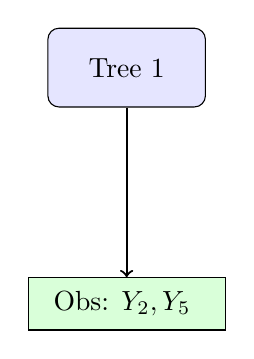
\begin{tikzpicture}[
  node distance=0.15cm,
  data/.style={rectangle, draw, align=center, fill=blue!10, minimum width=2cm, minimum height=1cm, rounded corners},
  leaf/.style={rectangle, draw, align=center, fill=green!15, minimum width=2.5cm, inner sep=5pt}
  ]
  
  \node[data] (root1) at (0, 3) {Tree 1};
  \node[leaf] (leaf1) at (0, 0) {
    Obs: $Y_2, Y_5$
  };
  \draw[->, thick] (root1) -- (leaf1);
\end{tikzpicture}
\end{columns}

\[
P(Y = y_2 \mid \mathbf{x}_{\text{new}}) = \frac{1}{2} \left( \frac{1}{3} + \frac{1}{2} \right) = \frac{5}{12}.
\]
}
\end{frame}


\begin{frame}{Inference and Prediction}
\note{
With this empirical probability function, we have flexibility for a variety of inferential statistics. For example, we can simulate new data, and also extract all the usual outputs that we would obtain from a standard random forest.

We are still exploring the use of this method to extract interesting inferential statistical results. However, we have also compared traditional prediction based on the mean function with other approaches.
}

The empirical conditional distribution:
\[
P(Y = y_i \mid X = \mathbf{x}_{\text{new}}) = w_i(\mathbf{x}_{\text{new}}), \quad i = 1, \dots, n.
\]

This allows easy computation of distributional quantities:

\begin{center}
\colorbox{green!10}{\parbox{0.5\textwidth}{
\begin{center}
\resizebox{\linewidth}{!}{%
     $\mathbb{E}(Y \mid X = \mathbf{x}_{\text{new}}) = \sum_{i=1}^{n} w_i(\mathbf{x}_{\text{new}})\, y_i$
}
\end{center}
}}
\end{center}

\begin{center}
\colorbox{green!10}{\parbox{0.5\textwidth}{
\begin{center}
\resizebox{\linewidth}{!}{%
 $P(Y \le y \mid X = \mathbf{x}_{\text{new}}) = \sum_{i: y_i \le y} w_i(\mathbf{x}_{\text{new}})$
}
\end{center}
}}
\end{center}
\end{frame}


% \begin{frame}{Improving Efficiency}
% I have worked to make the code more efficient, and it is already quite fast now. 
% To achieve even better performance, we can combine the following methods:

% \begin{enumerate}
%     \item \textbf{Distributed computing}
%     \item \textbf{Parallelisation}
%     \item \textbf{Vectorisation}
% \end{enumerate}
% \end{frame}